% !TEX root = ./Vorlesungsmitschrift DIFF 2.tex  
\chapter{Lebesgue-Integration}
\lecture{Do 25.10. 10:15}{}
Integralbegriff, \sd \( \Integrate{f_n}{x} \) \tto \( \Integrate{f}{x} \), wenn \( f_n\to f \) punktweise \( \rightsquigarrow \) Lebesgue-Integral. Unterschiedliche Zugänge. Hier: \emph{Riesz} (\href{https://arxiv.org/abs/1805.07289}{Vilmos Komornik, arXiv: 1805.07289}) \vgl auch Otto Forster, Analysis 3, Springer Vieweg, \emph{vor 2010}.

\begin{definition}
  Eine Teilmenge \( N\subset \reals^n \) heißt \emph{Nullmenge}, wenn es zu jedem \( \varepsilon>0 \) eine abzählbare Überdeckung von \( N \) durch offene Quader gibt mit Gesamtvolumen \( <\varepsilon \) (\( \volume{I_1\times \dotsb \times I_n}=\abs{I_1}\dotsm \abs{I_n} \)). Man sagt eine Eigenschaft träge \emph{fast überall} (\fue) zu, wenn sie außerhalb einer Nullmenge zutrifft.
\end{definition}
\begin{beispiele*}
  \begin{itemize}
    \item \( N=\bigcup_{i=1}^{\infty}\Set{x_i} \) ist Nullmenge \( \subset \reals \).
    \item \( \rationals \) ist Nullmenge \( \subset \reals \).
    \item \( f(x)=1 \), \( g(x)=\begin{cases}
      1 & c\neq 0 \\ 0 & x=0
    \end{cases} \), \( f=g \) \fue.
  \end{itemize}
\end{beispiele*}
Im Folgenden wollen wir Funktionen, die \fue gleich sind, miteinander identifizieren. Wir bilde also Äquivalenzklassen
\begin{equation*}
  \equivclass{f}=\Set{g|f=g \text{ \fue}}.
\end{equation*}
\begin{notation*}
  Wir schreiben dennoch \( f \) (nicht \( \equivclass{f} \)) und \( f=g \), \( \subseteq g \), \( f_n\to f \), \dots, wenn dies nur \fue gilt.
\end{notation*}
\begin{definition}\label{stufen_mit_integral}
  Eine Stufenfunktion ist eine Funktion der Form
  \begin{equation*}
    \varphi=\sum_{j=1}^{n}c_j \characteristicfunction;{Q},
  \end{equation*}
  \( Q_j=i_{j,1}\times\dotsb I_{j,n} \), \( I_{j,i} \) \emph{beschränkte} Intervalle.
  \begin{equation*}
    \characteristicfunction{Q}{x}=\begin{cases}
      1&x\in Q\\
      0& x\not\in Q
    \end{cases}
  \end{equation*}
  \enquote{charakteristische Funktion}. \emph{Integral} von \( \varphi \)
  \begin{equation*}
    \Integrate{\varphi}{x}\definedas \sum_{j=1}^{m}c_j \volume{Q_j}
  \end{equation*}
\end{definition}
\begin{lemma}
  \( \stufenfunktionen= \) Menge aller Stufenfunktionen (\bzw Äquivalenzklassen).
  \begin{itemize}
    \item \( \stufenfunktionen \) ist Vektorraum.
    \item \label{integral_aequivalente_stufenfunktionen_gleich}\( \Integrate{\varphi}{x} \) hängt nicht von der Wahl des Repräsentanten \( \varphi \) ab.
    \item \( \int\maps \stufenfunktionen \to \reals \), \( \varphi\mapsto \Integrate{\varphi}{x} \) ist linear und \( \Integrate{\varphi}{x}\geq 0 \), wenn \( \varphi\geq 0 \).
  \end{itemize}
\end{lemma}
\begin{proof}
  \vgl \diffcourse{1} (für \( Q=I \), hier genauso!), aber Achtung: Hier geht es um Äquivalenzklassen.
  \begin{proofdescription}
  \item[\ref{integral_aequivalente_stufenfunktionen_gleich}] folgt aus dem Satz von Borel (siehe unten): nicht-ausgeartete Intervalle (\( \neq \emptyset \), \( \neq \set{x} \)) sind keine Nullmenge in \( \reals \). Also sind nicht-ausgeartete Quader (also solche, die keine ausgearteten Intervalle enthalten) keine Nullmenge in \( \reals^n \). Nur nicht-ausgeartete Quader liefern  einen Beitrag zum Integral.
  \begin{subproof}
    \Obda \( I=\interval{0}{1} \) (den \( \set{0,1} \) ist Nullmenge). Angenommen, \texists  \( I_j \) offen \sd \( I\subset \bigcup I_j \) und \( \sum_{j=1}^{\infty}\abs{I_j}<\varepsilon \) mit \( 0<\varepsilon<1 \). \( \interval{0}{1} \) ist kompakt \timplies \texists \( i_1,\dotsc,i_k \) \sd
    \begin{equation*}
      \interval{0}{1}\subset \bigcup_{j=1}^k \mathcal{U}_{i_j}\implies 1=\Integrate{0}{1}{x}\explain{\sum_{j=1}^{k}\characteristicfunction{I_{i_j}}{x}\geq 1\ (\text{\diffcourse{1}})}{\leq}\Integrate{\sum_{j=1}^{k}\characteristicfunction{I_{i_j}}{x}}{x}\explain{\text{\diffcourse{1}}}{=}\sum_{j=1}^{k}\Integrate{\characteristicfunction{I_{i_j}{x}}}{x}<\varepsilon\ \contra.
    \end{equation*}    
  \end{subproof}
  \end{proofdescription}
  
\end{proof}
\begin{notation*}
  \( f_k(x)\goesupto f(x) \) oder \( f_k\goesupto f \) wenn \( f_k\goesto f \) punktweise (\fue)  und \( f_k\leq f_{k+1} \) (\fue).  \( f_k(x)\goesdownto f(x) \) oder \( f_k\goesdownto f \) wenn \( f_k\goesto f \) punkteweise (\fue)  und \( f_k\geq f_{k+1} \) (\fue).
\end{notation*}
\begin{lemma}
  \begin{itemize}
    \item \label{stufenfunktionen_zu_null_integrale_zu_null}\( \p*{\varphi_k}_k\subset \stufenfunktionen \), \( \varphi_k(x)\goesdownto 0 \). Dann gilt \( \Integrate{\varphi_k}{x}\goesdownto 0\).
    \item\label{stufenfunktionen_zu_funktion_integral_endlich_funktion_endlich} \( \p*{\varphi_k}_k\subset \stufenfunktionen \), \( \varphi_k(x)\goesupto g(x) \) und \( \sup \Integrate{\varphi_k}{x}<\infty \) \timplies \( f \) ist \fue endlich.
  \end{itemize}
\end{lemma}
\begin{proof}
  \begin{proofdescription}
    \item[\ref{stufenfunktionen_zu_null_integrale_zu_null}] \texists \( \interval{a}{b}^n \) und \texists \( M\geq 0 \) \sd \( \evaluateat{\varphi_1}{\interval{a}{b}} \) und somit alle \( \varphi_k \) durch \( M \) beschränkt sind und setzen \( \phi_1 \), somit alle \( \varphi_k \) außerhalb \( \interval{a}{b}^n \) gleich \( 0 \). Wähle nun Repräsentanten. \tforall  \( \varepsilon>0 \) \texists abzählbar viele offene Quader mit \( \sum_{j} \volume{Q_j}<\varepsilon \) \sd alle \( \evaluateat{\varphi_k}{\interval{a}{b}\setminus \bigcup_j Q_j} \) stetig sind 
    \begin{equation*}
      \implies \norm{\varphi_k}_{\infty,\interval{a}{b}^n\setminus \bigcup_j Q_j}\goesto 0\implies 0\leq \Integrate{\varphi_k}{x}\leq M\varepsilon+\varepsilon(b-a)^n
    \end{equation*}
    für \( k \) groß genug.
    \item[\ref{stufenfunktionen_zu_funktion_integral_endlich_funktion_endlich}] Ersetze \( \varphi_k\) durch \( \tilde{\varphi}_k=\varphi_k-\varphi_1 \) \timplies \( \tilde{\varphi_k}\geq 0 \). Wähle \( A>0 \) \sd \( A\geq \sup \Integrate{\tilde{\varphi}_k}{x} \). Setze zu \( \varepsilon>0 \)
    \begin{equation*}
        \mathcal{U}_{\varepsilon}\definedas \Set{x\in \reals^n|f(x)>\frac{A}{\varepsilon}}.
    \end{equation*}
    Wir sind fertig, wenn wir zeigen, dass \( \mathcal{U}_{\varepsilon} \) Nullmenge ist. Setze
    \begin{equation*}
      \mathcal{U}_{k,k}\definedas \Set{x|\tilde{\varphi}_k(x)>\frac{A}{\varepsilon}\geq \tilde{\varphi}_{k-1}}\quad (\tilde{\varphi}_0=0).
    \end{equation*}
    \timplies \( \mathcal{U_{\varepsilon,k}}\cap \mathcal{U}_{\varepsilon,j} \) (wegen Monotonie) und \( U_{\varepsilon}=\bigcup_k \mathcal{U}_{\varepsilon,k} \) (wobei \( \mathcal{U}_{\varepsilon,k} \) eine endliche Vereinigung von Quadern ist). Nur noch zu zeigen:
    \begin{equation*}
      \sum_{j=1}^{\infty}\sum_{j=1}^{l_k}\volume{Q_{k,j}}\leq \varepsilon.
    \end{equation*}
    Dies gilt dann
    \begin{equation*}
      \frac{A}{\varepsilon}\sum_{k=1}^{m}\sum_{j=1}^{l_k}\volume{Q_{k,j}}\explain{\text{\Def }\mathcal{U}_{\varepsilon,k}}{\leq}\braceannotate{\Integrate{\varphi_k \characteristicfunction{\mathcal{U}_{\varepsilon,k}}}{x}}{\Integrate{\varphi_k}{x,\mathcal{U}_{\varepsilon,k}}}\leq \Integrate{\varphi_m}{x}\leq A.
    \end{equation*}
  \end{proofdescription}
  
\end{proof}
\begin{definition}\label{integral_stufen_hoch}
  \begin{equation*}
    \stufenfunktionen[1]\definedas \Set{f\maps \reals^n\to \compactification{\reals}=\reals\cup \set{\pm \infty}|\exists \p*{\varphi_k}_k\subset \stufenfunktionen,\quad \varphi_k(x)\goesupto f(x)}
  \end{equation*}
  zu \( f_1\in \stufenfunktionen[1] \) setzte \( \Integrate{f}{x}\definedas \lim_{k \goesto \infty}\Integrate{\varphi_k}{x}\in \compactification{\reals} \).
\end{definition}
\begin{satz}\label{integral_stufen_hoch_eigenschaften}
  \begin{enumerate}
    \item \label{integral_stufen_hoch_unabhaengig_von_stufenfolge}\( \int f \) wie in \ref{integral_stufen_hoch} ist unabhängig von der gewählten Folge \( \p*{\varphi_k}_k\subset \stufenfunktionen \).
    \item \label{integral_stufen_hoch_gleich_stufenintegral} Für \( f\in \stufenfunktionen \) stimmt der Integralbegriff mit dem aus \ref{stufen_mit_integral} überein.
    \item \label{integral_stufen_hoch_funktionenungleichung_integralungleichung} Sind \( f,g\in \stufenfunktionen[1] \) mit \( f\leq g \) so ist \( \int f\leq \int g \).
    \item \label{integral_stufen_hoch_linear} Sind \( g,f\in \stufenfunktionen[1] \), \( c\geq 0 \) so ist \( cf,f+g\in \stufenfunktionen[1] \) und \( \Integrate{cf}{x}=c\Integrate{f}{x} \), \( \Integrate{f+g}{x}=\Integrate{f}{x}+\Integrate{g}{x} \).
  \end{enumerate}
\end{satz}
Für den Beweis benötigen wir ein Lemma.
\begin{lemma}\label{funktionenungleichung_grenzwertungleichung_stufenfunktionen_hoch_zu}
  \( \p*{\varphi_k}_k,\p*{\psi_k}_k\subset \stufenfunktionen[0] \), \( \varphi_k\goesupto f \), \( \psi_k\goesupto g \). Ist \( f\leq g \), so gilt
  \begin{equation*}
    \lim_k \Integrate{\varphi_k}{x}\leq \lim_k \Integrate{\psi_k}{x}.
  \end{equation*}
\end{lemma}
\begin{proof}
  Es genügt zu zeigen: Für jedes \( m \) gilt
  \begin{equation*}
    \Integrate{\varphi_m}{x}\leq \lim \Integrate{\varphi_k}{x}.
  \end{equation*}
  Das ist äquivalent zu
  \begin{equation*}
    \lim_{h \goesto 0}\Integrate{\varphi_m-\varphi_k}{x}\leq 0.
  \end{equation*}
  Definiere
  \begin{equation*}
    \p*{\varphi_m-\varphi_k}^{+}\definedas \Max{\varphi_m-\varphi_k,0}\goesdownto 0 \quad (k\goesto \infty)
  \end{equation*}
  punktweise. \ref{stufenfunktionen_zu_null_integrale_zu_null} \timplies \( \lim_{k\goesto \infty}\Integrate{\p*{\varphi_m-\varphi_k}^{+}}{x}\goesdownto 0 \) \timplies \Beh.
\end{proof}
\approxtimestamp{33}
\begin{proof}[Beweis von \ref{integral_stufen_hoch_eigenschaften}]
  \begin{proofdescription}
    \item[\ref{integral_stufen_hoch_unabhaengig_von_stufenfolge}] folgt aus \ref{funktionenungleichung_grenzwertungleichung_stufenfunktionen_hoch_zu} mit \( f=g \).
    \item[\ref{integral_stufen_hoch_funktionenungleichung_integralungleichung}] folgt aus \ref{funktionenungleichung_grenzwertungleichung_stufenfunktionen_hoch_zu}. 
    \item[\ref{integral_stufen_hoch_linear}] \( \varphi_k\goesupto f \), \( \psi_k\goesupto g \) \timplies \( c\varphi_k\goesupto cf \), \( \varphi_k+\psi_k\goesupto f+g \). Der Rest folgt aus der Linearität der Integrals auf \( \stufenfunktionen \). 
  \end{proofdescription}
\end{proof}
\begin{bemerkung*}
  Achtung! Da wir \( \int f=\infty \) zulassen, kann man nicht einfach Linearität zeigen.
\end{bemerkung*}
\begin{beispiel*}
  \( \int f= \infty \), \( \int g=\infty \), \( \int (f-g)\neq 0 \) \ia.
\end{beispiel*}
\begin{konvention*}
  \( 0\cdot (\infty)=0 \), \( a+\infty=\infty \), \( a\cdot(\infty)=\infty \) (\( a>0 \)), \( a\cdot(\infty)=-\infty \) (\( a<0 \)). Konsistent mit \ref{integral_stufen_hoch_linear}.
\end{konvention*}
\begin{bemerkung*}
  Sind \( f,g\in \stufenfunktionen[1] \), so auch \( \funcmin{f,g} \) und \( \funcmax{f,g} \).
\end{bemerkung*}
\begin{proof}
  \begin{align*}
    \Min{f,g}=\frac{1}{2}(f+g-\abs{f-g})\\
    \Max{f,g}=f+g-\frac{1}{2}\abs{f-g}.
  \end{align*}
  
\end{proof}
\begin{lemma}\label{r1_hoch_zu_funktion_r1_integral_hoch_zu}
  \( \p*{f_k}\subset \stufenfunktionen[1] \), \( f_k\goesupto f \). Dann ist \( f\in \stufenfunktionen[1] \) und 
  \begin{equation*}
    \Integrate{f_k}{x}\goesupto \Integrate{f}{x}.
  \end{equation*}
\end{lemma}
\begin{proof}
  Zu \( k \) wähle \( \p*{\varphi_{k,j}}_i\subset \stufenfunktionen \) mit \( \varphi_{k,j}\goesupto_{j}f_k \). Dann ist für \( \varphi_i\definedas \sup_{k,j\leq i}\varphi_{k,j} \)
  \begin{equation*}
    \varphi_{i+1}\geq \varphi_i
  \end{equation*}
und für jedes feste \( k \) gilt
\begin{gather*}
  \varphi_{k,j}\leq \varphi_j\leq f \quad \forall j\geq k\\
  \implies f_k=\lim_{j \goesto \infty}\varphi_{k,j}\leq \lim_{j \goesto \infty}\leq f
\end{gather*}
\timplies (Sandwich-Lemma) \( \varphi_j\goesupto f \) \timplies \( f\in \stufenfunktionen[1] \) und \( \Integrate{\varphi_j}{x}\goesto \Integrate{f}{x} \). Wegen \( \varphi_k\leq f_k\leq f \) (nach Definition) folgt \Beh.
\end{proof}
\timestamp{42:15}
\begin{bemdef}
  Wir erweitern den Integralbegriff noch weiter: Ist \( f\in \stufenfunktionen[1] \), definiert man \( \Integrate{-f}{x}\definedas -\Integrate{f}{x} \).

  Allgemein: Sind \( f_1,f_2\in \stufenfunktionen[1] \) und \( \Integrate{f_1}{x}-\Integrate{f_2}{x} \) (ist definiert (\dh mindestens eines der Integrale ist endlich) dann ist \( f\definedas f_1-f_2 \) wohldefiniert (denn nach \ref{stufenfunktionen_zu_funktion_integral_endlich_funktion_endlich} ist dann eine der Funktionen \fue endlich). Die Menge all dieser FUnktionen \( f \) nennen wir \( \stufenfunktionen[2] \) und setze für \( f=f_1-f_2\in \stufenfunktionen[2] \), \( f_i\in \stufenfunktionen[1] \):
  \begin{equation*}
    \Integrate{f}{x}\definedas \Integrate{f_1}{x}-\Integrate{f_2}{x}.
  \end{equation*}
\end{bemdef}
\begin{bemerkung*}
  Ohne Einschränkung können wir annehmen, dass \( f_1,f_2\geq 0 \) (sonst wähle \( \phi,\psi\in \stufenfunktionen[0] \) mit \( \varphi\leq f_1 \) und \( \psi\leq f_2 \) und betrachte \( f_1-\Min{\phi,\leq} \) und \( f_2-\Min{\varphi,\psi} \)).
  \begin{figure}[H]
    \centering
    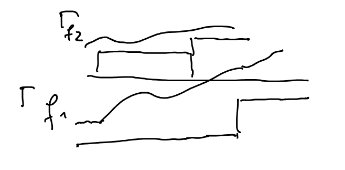
\includegraphics[width=0.5\linewidth]{r1_funktionen_nach_unten_beschraenkt}
    \label{fig:r1_funktionen_nach_unten_beschraenkt}
  \end{figure}
  \begin{equation*}
    f=f_1-\Min{\varphi,\psi}-(f_2-\Min{\varphi,\psi})=f_1-f_2.
  \end{equation*}
\end{bemerkung*}
\begin{satz}\label{r2_eigenschaften}
  \( f\in \stufenfunktionen[2] \)
  \begin{enumerate}
    \item \label{integral_r2_unabhaengig_von_r1_wahl} \( \Integrate{f}{x} \) ist unabhängig von der Wahl von \( f_1,f_2 \)
    \item \label{integral_r2_stimmt_mit_integral_r1_ueberein} Ist \( f\in \stufenfunktionen[1]\subset \stufenfunktionen[2] \), stimmt \( \Integrate{f}{x} \) mit dem Integral auf \( \stufenfunktionen[1]\) (\ref{integral_stufen_hoch}) überein.
    \item \label{integral_r2_monotonie} Monotonie: Sind \( f,g\in \stufenfunktionen[2] \), \( f\leq g \) so ist \( \Integrate{f}{x}\leq \Integrate{g}{x} \).
    \item \label{summe_r2} Sind \( f,g\in \stufenfunktionen[2] \) und \( \Integrate{f}{x}+\Integrate{g}{x} \) ist definiert, so ist \( f+g\in \stufenfunktionen[2] \) und \( \Integrate{f+g}{x}=\Integrate{f}{x}+\Integrate{g}{x} \).
    \item \label{skalarmultiplikation_r2} Ist \( f\in \stufenfunktionen[2] \), \( c\in \reals \), so ist \( cf\in \stetigefunktionen[2] \) und \( \Integrate{cf}{x}=c\Integrate{f}{x} \).
  \end{enumerate}
\end{satz}
\begin{proof}
  \begin{proofdescription}
    \item[\ref{integral_r2_unabhaengig_von_r1_wahl} und \ref{integral_r2_monotonie}] Wir zeigen: Wenn \( f=f_1-f_2 \) und \( g=g_1-g_2 \) und \( f\leq g \), dann gilt:
    \begin{equation*}
      \tag{\( * \)} \Integrate{f_1}{x}-\Integrate{f_2}{x}\leq \Integrate{g_1}{x}-\Integrate{g_2}{x}\label{r2_funktionen_ungleichung_integral_ungleichung}
    \end{equation*}
    (daraus folgt \ref{integral_r2_unabhaengig_von_r1_wahl} mit \( f=g \)). Fallunterscheidungen:
    \begin{eigenschaftenenumerate}[ref=\rechtsklammer{\alph*}]
      \item Ist \( \Integrate{f_2}{x}=\infty \) so gilt \eqref{integral_r2_unabhaengig_von_r1_wahl}.
      \item\label{r2_funktionen_ungleichung_integral_ungleichung:beide_endlich} Ist \( \Integrate{f_2}{x}<\infty \) und \( \Integrate{g_1}{x}<\infty \), so sind \( f_2 \) und \( g_2 \) endlich \fue (\ref{stufenfunktionen_zu_funktion_integral_endlich_funktion_endlich}) \timplies \( f_1+g_2\leq g_1+f_2 \) (wegen \( f_1-f_2\leq g_1-g_2 \)) \timplies \( \int f_1+\int g_2\leq \int g_1+\int f_2 \) (\ref{integral_stufen_hoch_linear}) \timplies \eqref{integral_r2_unabhaengig_von_r1_wahl}.
      \item Ist \( \Integrate{f_2}{x}<\infty \) und \( \Integrate{g_2}{x}=\infty \), wähle \( \p*{\varphi_k}_k\subset \stufenfunktionen[0] \) mit \( \varphi_k\goesupto g_2 \). Dann ist \( f_1-f_2\leq g_1-\varphi_k \quad \forall k \). Wende \ref{r2_funktionen_ungleichung_integral_ungleichung:beide_endlich} auf \( f_1,f_2,g_1,\varphi_k \) an \timplies \( \int f_1-\int f_2\leq \int g_1-\int \varphi_k \) \timplies \eqref{r2_funktionen_ungleichung_integral_ungleichung} (\( k\goesto \infty \)).
    \end{eigenschaftenenumerate}
    \item[\ref{integral_r2_stimmt_mit_integral_r1_ueberein}] Folgt aus \ref{integral_r2_unabhaengig_von_r1_wahl} mit \( f_1\definedas f \), \( f_2\definedas 0 \).
    \item[\ref{skalarmultiplikation_r2}] Folgt aus der Definition in wie in \ref{integral_stufen_hoch_linear}
    \item[\ref{summe_r2}] Schreibe \( f=f_1-f_2 \), \( g=g_1-g_2 \) mit \( f_1,f_2,g_1,g_2\in \stufenfunktionen[1] \).  
    \begin{eigenschaftenenumerate}[ref=\rechtsklammer{\alph*}]
      \item \label{summe_r2:beide_endlich} Ist \( \Integrate{f_2}{x}<\infty \), \( \Integrate{g_2}{x}<\infty \), \( f_1+g_2, f_2+g_2\in \stufenfunktionen[1] \) (\ref{integral_stufen_hoch_linear})  und \( \Integrate{f_2+g_2}{x}=\Integrate{f_2+g_2}{x}<\infty \)
      \begin{equation*}
        \implies f+g=(f_1+g_2)-(f_2+g_2)\in \stetigefunktionen[2]
      \end{equation*}
      und 
      \begin{align*}
        \Integrate{f+g}{x}=\Integrate{f_1+g_2}{x}-\Integrate{f_2+g_2}{x}\\
        &=\int f_1+\int g_1-\int f_2-\int g_2\\
        &=\int f+\int g.
      \end{align*}
      \item Ist \( \int f_2=\infty \) oder \( \int g_2=\infty \), so sind \emph{beide Integrale \( \int f_1,\int g_1 \) endlich}. Denn \( f,g\in \stufenfunktionen[2] \) und wir hatten vorausgesetzt, dass \( \Integrate{f}{x}+\Integrate{g}{x} \) definiert ist. Wir können also Beweis \ref{summe_r2:beide_endlich} wiederholen. \(\int f_2=\infty\) \timplies \( \int f_1<\infty \) und \( \int g <\infty \)).
    \end{eigenschaftenenumerate}
  \end{proofdescription}
  
\end{proof}
\begin{satz}[Verallgemeinerter Satz von Beppo-Levi] \label{beppo-levi}
  Sei \( \p*{f_k}_k\subset \stetigefunktionen[2] \), \( f_k\goesupto f \). Ist \( \Integrate{f_k}{x}>-\infty \) für ein \( k \), so ist \( f\in \stufenfunktionen[2] \) und 
  \begin{equation*}
    \label{eq:beppo-levi} \Integrate{f_k}{x}\goesupto \Integrate{f}{x}\tag{\( * \)}.
  \end{equation*}
\end{satz}
\begin{bemerkung*}
  Die Voraussetzung ist wichtig:\\
  Betrachte \( f_k=-\characteristicfunction.{\ointerval{-\infty}{0}}{}+\characteristicfunction.{\ointerval{0}{k}}{} \). Dann ist \( f=\sgn;\not\in \stufenfunktionen[2] \), \( \sgn{x}=\begin{cases}
    1&x>0\\ 0&x=0\\ -1&x<0.
  \end{cases} \)
  Betrachte \( f_k=-\characteristicfunction-{\ointerval{k}{\infty}}{} \). Dann ist \( f=0\in \stufenfunktionen[2] \) aber \eqref{eq:beppo-levi} trifft nicht zu.
\end{bemerkung*}
\begin{proof}[Beweis von \ref{beppo-levi}]
  Für \( k\geq k_0 \) gilt \( \int f_k>-\infty \) (wegen der Monotonie). Sei \( k\geq k_0 \). Schreibe \( f_k=g_k-h_k \), \( g_k,h_k\in \stufenfunktionen[1] \). Dann ist \( \int h_k<\infty \) \timplies \texists \( \varphi_k\in \stufenfunktionen[0] \) \sd \( \varphi_k\leq h_k \) und \( \Integrate{h_k-\varphi_k}{x}<2^{-k} \)
  \begin{equation*}
    \implies f_k=\p{\braceannotate{=\tilde{g_k}}{g_k-\varphi_k}}-\p{\braceannotate{\tilde{h}_k}{h_k-\varphi_k}}
  \end{equation*}
  und es gilt \( \tilde{h}_k\geq 0 \) und \( \int \tilde{h}_k<2^{-k} \), \( \tilde{h}_k,\tilde{g}_k\in \stetigefunktionen[1] \).
  Schreibe nun
  \begin{equation*}
    f_k=(\tilde{h}_1+\dotsb+\tilde{h}_{k-1}+\tilde{g_k})-(\tilde{h}_1+\dotsc+\tilde{h}_{k-1}+\tilde{h}_k)=G_k-H_k
  \end{equation*}
  mit \( H_k,G_k\in \stufenfunktionen[1] \), \( \int H_k\leq 1 \). \thref{r1_hoch_zu_funktion_r1_integral_hoch_zu} \timplies \( G_k\goesupto G \), \( H_k\goesupto H \) mit \( G,H\in \stufenfunktionen[1] \) und \( \int H\leq 1 \)
  \begin{equation*}
    \implies f=G-H\in \stufenfunktionen[2]
  \end{equation*}
  und
  \begin{equation*}
    \Integrate{f_k}{x}=\Integrate{G_k}{x}-\Integrate{H_k}{x}\goesto \Integrate{G}{x}-\Integrate{H}{x}=\Integrate{f}{x}.
  \end{equation*}
\end{proof}
\begin{folgerung*}\label{max_min_von_r2_ist_r2}
  \( f,g\in \stufenfunktionen[2] \) \timplies \( \funcmax{f,g},\funcmin{f,g}\in \stetigefunktionen[2] \).
\end{folgerung*} 
\begin{proof}[Beweis (nur für \( \max \))]
  Seien \( f=f_1-f_2 \), \( g=g_1-g_2 \).
  \begin{eigenschaftenenumerate}
    \item\label{max_min_von_r2_ist_r2:stufenfunktionen} \( f_1,g_1\in \stufenfunktionen[0] \) \timplies \( \Integrate{f_1+g_1}{x}<\infty \) und 
    \begin{align*}
      \funcmax{f_1-f_2,g_1-g_2}&=(f_1+g_1)+\funcmax{-g_1-f_2,-f_1-g_2}\\
      &=\p*{\braceannotate{\in \stufenfunktionen[1]}{f_1+g_1}}-\braceannotate{\in \stetigefunktionen[1]}{\min{g_1+f_1,f_1+g_2}}.
    \end{align*}
    \item \( \int f_1+g_1<\infty \) \timplies \( \funcmax{f_1-f_2,g_1,g_1-g_2}\in \stufenfunktionen[2] \). \( f_1,g_1\not\in \stufenfunktionen[0] \), wähle \( \varphi_k\goesupto f_1 \), \( \leq_k\goesupto g_1 \).  \ref{max_min_von_r2_ist_r2:stufenfunktionen} \timplies \( \Integrate<{\funcmax{\varphi_k-f_2,\psi_k-g_2}}{x} >-\infty\quad \forall  k\), weil \( \Integrate{f_2}{x}<\infty \) oder \( \Integrate{g_2}{x}<\infty \) \timplies \Beh aus Beppo-Levis Satz.
  \end{eigenschaftenenumerate}
\end{proof}